% ==============================================================================
% Refined Sections 1, 2, 3, 4 for Laboratory 1 Report
% Author: CCDS Lab 1 Group
% Sections covered:
%   1. Introduction
%   2. Architecture (to be reviewed next)
%   3. Images and design decisions (to be reviewed next)
%   4. Scalability and high availability (to be reviewed next)
% ==============================================================================

\documentclass[11pt,a4paper]{article}
\usepackage[T1]{fontenc}
\usepackage{lmodern}
\usepackage[margin=2.2cm]{geometry}
\usepackage{booktabs,tabularx,enumitem,listings,xcolor,array}
\usepackage{longtable}
\usepackage{tikz}
\usetikzlibrary{positioning,fit,backgrounds,arrows.meta,calc}
\usepackage[hidelinks]{hyperref}

\lstset{basicstyle=\ttfamily\small,backgroundcolor=\color{gray!8},frame=single,
        rulecolor=\color{gray!40},breaklines=true,columns=fullflexible}
\setlist{nosep}
\newcommand{\svc}[1]{\texttt{#1}}
\newcolumntype{Y}{>{\raggedright\arraybackslash}X}

\definecolor{cfront}{HTML}{DDE7FF}
\definecolor{capp}{HTML}{DFF5E1}
\definecolor{cstats}{HTML}{FFF1CC}
\definecolor{catenea}{HTML}{FFE0E0}
\definecolor{cbackup}{HTML}{E8DEFF}

\sloppy
\begin{document}

\section{Introduction}

We containerised the infrastructure outlined in the laboratory assignment: the shared services
(\emph{basic}), a company application (\emph{app}), an observability platform
(\emph{stats}), and Moodle (\emph{atenea}). For the core application, we developed a reviews
service in Flask: users can post comments with a 1-to-5 rating, view score distributions and
recent reviews, trigger email notifications through an internal SMTP relay upon each submission,
and ingest external ratings via an automated background feeder.

The implementation is designed for production-grade resilience: every user-facing component
maintains at least two replicas distributed across distinct nodes, the application database
and caching layers are clustered with automatic failover, backups are encrypted and stored on
a dedicated node, and all services export health and telemetry metrics. Deployment is
fully automated, requiring only a single \texttt{docker compose up} for local execution or
\texttt{docker stack deploy} for production Swarm orchestration, using pre-built images published
to Docker Hub.

The repository is organised into \texttt{compose.yml} (local), \texttt{production.yml} (Swarm),
service directories containing their respective \texttt{Dockerfile} definitions and runtime
assets, helper automation in \texttt{scripts/} (node labelling, image publishing, Swarm simulation,
and disaster recovery), and this report. The local environment operates without TLS and uses
named volumes, yet preserves the exact clustering topology present in production to enable verification on a single development machine.

\section{Architecture}

\subsection{Nodes}

The swarm comprises seven nodes; service placement is controlled via the Docker Swarm node label \texttt{role}
(along with \texttt{slot} on the application nodes to enforce separation between primaries and replicas).

\begin{figure}[ht]
\centering
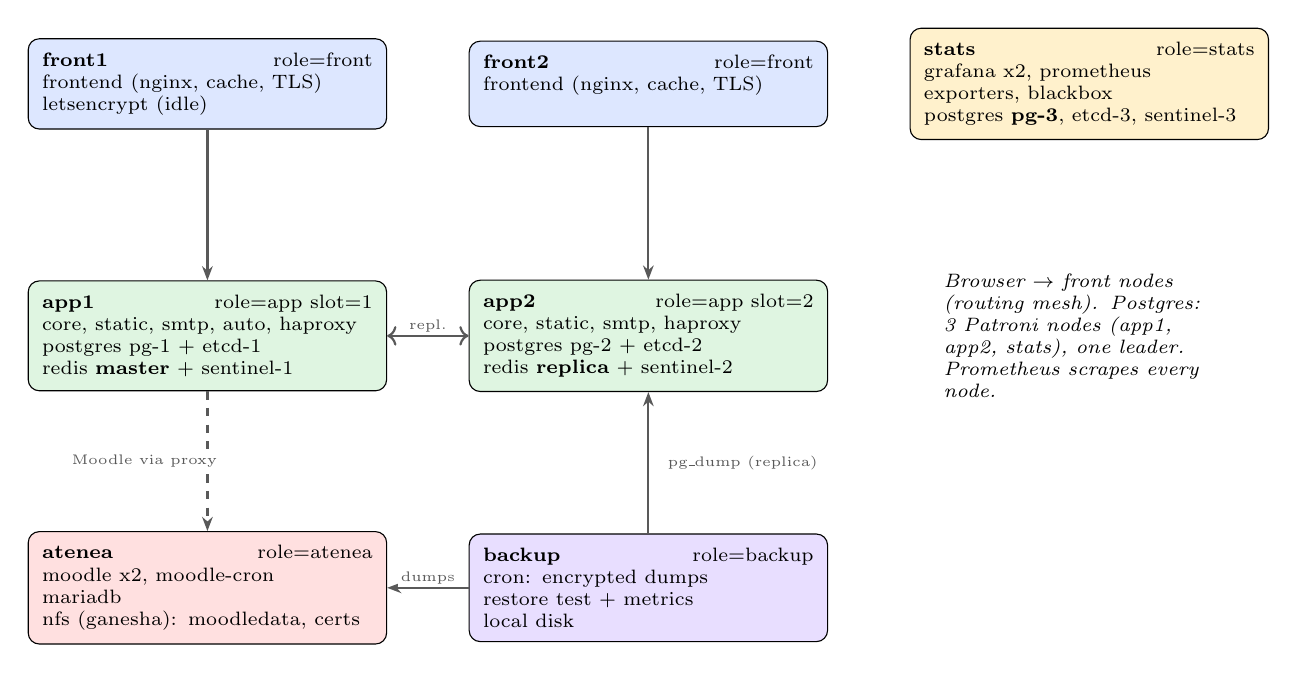
\begin{tikzpicture}[
  vm/.style={draw,rounded corners=4pt,text width=4.2cm,align=left,inner sep=5pt,font=\scriptsize},
  arr/.style={-{Stealth[length=1.8mm]},thick,gray!70!black},
  lab/.style={font=\tiny,fill=white,inner sep=1pt}]
\node[vm,fill=cfront]  (f1) at (0,0)    {\textbf{front1} \hfill role=front\\ frontend (nginx, cache, TLS)\\ letsencrypt (idle)};
\node[vm,fill=cfront]  (f2) at (5.6,0)  {\textbf{front2} \hfill role=front\\ frontend (nginx, cache, TLS)\\ \phantom{x}};
\node[vm,fill=cstats]  (st) at (11.2,0) {\textbf{stats} \hfill role=stats\\ grafana x2, prometheus\\ exporters, blackbox\\ postgres \textbf{pg-3}, etcd-3, sentinel-3};
\node[vm,fill=capp]    (a1) at (0,-3.2)   {\textbf{app1} \hfill role=app slot=1\\ core, static, smtp, auto, haproxy\\ postgres pg-1 + etcd-1\\ redis \textbf{master} + sentinel-1};
\node[vm,fill=capp]    (a2) at (5.6,-3.2) {\textbf{app2} \hfill role=app slot=2\\ core, static, smtp, haproxy\\ postgres pg-2 + etcd-2\\ redis \textbf{replica} + sentinel-2};
\node[vm,fill=catenea] (at) at (0,-6.4)   {\textbf{atenea} \hfill role=atenea\\ moodle x2, moodle-cron\\ mariadb\\ nfs (ganesha): moodledata, certs};
\node[vm,fill=cbackup] (bk) at (5.6,-6.4) {\textbf{backup} \hfill role=backup\\ cron: encrypted dumps\\ restore test + metrics\\ local disk};
\node[font=\scriptsize\itshape,text width=3.7cm,align=left] at (11.2,-3.2) {Browser $\to$ front nodes (routing mesh). Postgres: 3 Patroni nodes (app1, app2, stats), one leader. Prometheus scrapes every node.};
\draw[arr] (f1) -- (a1);
\draw[arr] (f2) -- (a2);
\draw[arr,<->] (a1) -- node[lab,above]{repl.} (a2);
\draw[arr,dashed] (a1) -- node[lab,pos=.5,xshift=-8mm]{Moodle via proxy} (at);
\draw[arr] (bk) -- node[lab,pos=.5,xshift=12mm]{pg\_dump (replica)} (a2);
\draw[arr] (bk) -- node[lab,above]{dumps} (at);
\end{tikzpicture}
\caption{Nodes and services (simplified). The routing mesh accepts the traffic on both front
nodes; \svc{backup} pulls from a replica, from MariaDB and from the NFS volume.}
\label{fig:nodes}
\end{figure}

\subsection{Services}

Table~\ref{tab:services} maps the components from the assignment specification to our implemented services,
the nodes where they run, and their replica counts. Each stack operates within an encrypted overlay network,
and each service only joins the networks it strictly requires: for instance, the databases do not participate
in the \texttt{proxy} network, ensuring they remain isolated and inaccessible from the frontend.

\begin{table}[ht]
\centering\small
\begin{tabularx}{\textwidth}{llllY}
\toprule
Stack & Service & Nodes & Repl. & Description \\
\midrule
basic  & \svc{frontend}    & front   & 2 & nginx: only public service (80/443), cache, TLS, proxy by subdomain \\
       & \svc{letsencrypt} & front   & 1 & certbot; idle with a local domain (self-signed certificate) \\
       & \svc{nfs}         & atenea  & 1 & NFSv4 server (NFS-Ganesha) inside the stack, port 2049 in host mode \\
\midrule
app    & \svc{core}        & app     & 2 & Flask + gunicorn, reviews \\
       & \svc{static}      & app     & 2 & Apache httpd, \texttt{/static/} \\
       & \svc{pg-1..3}    & app1, app2, stats & 3 & PostgreSQL 16 + Patroni (leader + 2 replicas) \\
       & \svc{etcd-1..3}   & app1, app2, stats & 3 & consensus store of Patroni \\
       & \svc{db}          & app     & 2 & HAProxy: \texttt{db:5432} leader, \texttt{db:5433} replicas \\
       & \svc{redis-1}, \svc{redis-2} & app1, app2 & 1+1 & cache: master and replica \\
       & \svc{sentinel-1..3} & app1, app2, stats & 3 & failover of the cache (quorum 2) \\
       & \svc{smtp}        & app     & 2 & Postfix relaying the mails (to Mailpit by default) \\
       & \svc{mailpit}     & app     & 1 & mail catcher with a web page (\texttt{mail.localhost:8080}) \\
       & \svc{auto}        & app     & 1 & feeder of external ratings \\
       & \svc{backup}      & backup  & 1 & encrypted dumps + restore test \\
\midrule
atenea & \svc{moodle}      & atenea  & 2 & Moodle 4.5.14 LTS \\
       & \svc{moodle-cron} & atenea  & 1 & same image, \texttt{cron.php} every minute \\
       & \svc{moodle-db}   & atenea  & 1 & MariaDB 11.4 \\
\midrule
stats  & \svc{grafana}     & stats   & 2 & dashboards as code + Infinity plugin (the ``?'') \\
       & \svc{prometheus}  & stats, backup & 2 & metrics and alert rules, one TSDB per replica \\
       & exporters         & stats / global & --- & postgres, redis, mysqld, nginx, blackbox, node, cAdvisor \\
\bottomrule
\end{tabularx}
\caption{Services of the infrastructure.}
\label{tab:services}
\end{table}

Public entrypoints in production are exposed via \texttt{app.<domain>}, \texttt{lms.<domain>}, and
\texttt{grafana.<domain>}; with the default \texttt{DOMAIN=localhost}, they resolve to
\texttt{app.localhost}, \texttt{lms.localhost}, and \texttt{grafana.localhost} on port 443. Locally, the same names are served on port 8080 over HTTP (modern browsers resolve \texttt{*.localhost} to 127.0.0.1 automatically).

\section{Images and design decisions}

\paragraph{Frontend and caching.} We use \texttt{nginx:alpine} as the single public entrypoint for all services. Nginx terminates TLS, routes subdomains to their internal services, and caches dynamic pages for 10~seconds and static files for one hour. When a user submits a review, a temporary cookie bypasses the cache so their new comment appears immediately. The page footer displays which frontend and application nodes handled the request, demonstrating load distribution across replicas.

\paragraph{TLS and certificates.} Production exposes HTTPS on port 443 using a self-signed certificate generated at container startup, allowing Nginx to boot without external dependencies. The \svc{letsencrypt} service is fully defined in the stack with automated renewal logic, but remains idle when running with local domains (\texttt{localhost}) where public certificate authorities cannot validate ownership.

\paragraph{Core application.} The reviews application is built with Python 3.12 and runs as a non-root user with two replicas. To maintain high performance, page data is cached in Redis with version-based invalidation upon new submissions. The application degrades gracefully: if Redis is unreachable, requests fall back directly to the database; if the database is temporarily recovering, the service returns a clean HTTP 503 instead of crashing. Database operations are decoupled via HAProxy: writes target the leader (port 5432) while reads are distributed across replicas (port 5433).

\paragraph{PostgreSQL cluster (Patroni).} Database high availability is managed by Patroni across three PostgreSQL 16 nodes (\svc{pg-1}, \svc{pg-2}, \svc{pg-3}) distributed over \texttt{app1}, \texttt{app2}, and \texttt{stats}. A three-node etcd cluster provides distributed consensus for leader election and health tracking. If the active leader fails, Patroni automatically promotes a replica within seconds. HAProxy (\svc{db}) sits in front of the cluster, continuously querying Patroni's health API to expose consistent endpoints (\texttt{db:5432} for writes, \texttt{db:5433} for reads) so application services require no configuration changes during a failover.

\paragraph{Redis cache and Sentinel.} Redis caching uses a primary-replica architecture paired with three Redis Sentinels across separate nodes (quorum of 2). The application dynamically discovers the active master through Sentinel, enabling automatic failover if the primary node goes offline.

\paragraph{Moodle LMS.} Moodle 4.5 LTS is deployed using PHP 8.3 Apache with two replicas. On initial launch, an automated script runs the command-line installer, utilizing a filesystem lock in the shared volume to prevent race conditions between containers. User sessions are persisted in MariaDB, allowing any replica to serve incoming requests interchangeably. A dedicated container (\svc{moodle-cron}) runs scheduled tasks in the background.

\paragraph{Shared storage (NFS).} Because Docker Swarm restricts privileged containers on worker nodes, we deploy \textbf{NFS-Ganesha} in user space on the \texttt{atenea} node. It exports shared volumes for Moodle data and certificates using only standard Linux capabilities, enabling seamless multi-node file sharing without requiring kernel-level NFS modules on the host.

\paragraph{Backups and observability.} See Sections~\ref{sec:backup} and~\ref{sec:obs}.

\paragraph{Scope of production.} In the context of this project, ``production'' represents the complete multi-node Swarm architecture running on local Docker-in-Docker nodes. Because it is evaluated locally rather than on a public cloud provider, services use \texttt{localhost} subdomains and self-signed certificates.

\section{Scalability and high availability}

\subsection{Replicas}

The project guidelines require all services to be scalable, excluding periodic jobs and non-distributed DBMS. Stateless components (\svc{frontend}, \svc{core}, \svc{static}, \svc{db}, \svc{smtp}, \svc{grafana}, \svc{moodle}, and \svc{prometheus}) are deployed with two replicas and can be dynamically scaled using \texttt{docker service scale}. Prometheus automatically discovers active replicas via Docker Swarm DNS (\texttt{tasks.<service>}).

Services intentionally kept at a single replica include periodic background jobs (\svc{letsencrypt}, \svc{backup}, \svc{moodle-cron}, and \svc{auto}, where duplicate runs would be redundant), single-host storage (\svc{nfs}), developmental tooling (\svc{mailpit}), and \svc{moodle-db}. The primary stateful layers (PostgreSQL and Redis) are not scaled naively, but are deployed as high-availability clusters with automated leader election and replication.

\subsection{Failures}

Table~\ref{tab:failures} summarizes the system resilience matrix, categorizing the direct impact, mitigation mechanism, and recovery process across service-level and node-level outages.

\begin{table}[ht]
\centering\small
\begin{tabularx}{\textwidth}{l p{3.6cm} Y l}
\toprule
\textbf{Failure Target} & \textbf{Direct Impact} & \textbf{Mitigation Mechanism} & \textbf{Recovery} \\
\midrule
\multicolumn{4}{l}{\textit{\textbf{Service / Container Failures}}} \\
\addlinespace[2pt]
Frontend replica & None & Swarm routing mesh directs traffic to survivor & Automatic \\
Core / static replica & None (transparent) & Nginx serves stale cache; Swarm reschedules & Automatic \\
Redis master & Brief cache miss spike & Sentinels promote replica; app degrades gracefully & Automatic ($<$5\,s) \\
Postgres leader & Brief write pause & Patroni elects replica; HAProxy reroutes traffic & Automatic ($<$3\,s) \\
\midrule
\multicolumn{4}{l}{\textit{\textbf{Node Outages}}} \\
\addlinespace[2pt]
\texttt{front1} or \texttt{front2} & None & Routing mesh routes via surviving front node & Automatic \\
\texttt{app1} or \texttt{app2} & Reduced capacity & App2 serves; Patroni/Redis failover; etcd 2/3 quorum & Automatic \\
\texttt{stats} & Metrics interrupted & Core app unaffected; etcd/Patroni maintain 2/3 quorum & On node restart \\
\texttt{atenea} & Moodle \& NFS down & Core app unaffected; TLS certs cached in Nginx & On node restart \\
\texttt{backup} & Backup jobs pause & User-facing services completely unaffected & On node restart \\
\bottomrule
\end{tabularx}
\caption{System resilience and failure recovery matrix.}
\label{tab:failures}
\end{table}

\subsection{Updates}

Updates are applied one container at a time (\texttt{parallelism: 1}, \texttt{order: stop-first}) with automated rollback upon error (\texttt{failure\_action: rollback}). Each custom image includes a defined \texttt{HEALTHCHECK}, guaranteeing that an updated replica is verified healthy before the deployment progresses to the next node. Furthermore, stateless services enforce \texttt{max\_replicas\_per\_node: 1}, ensuring replicas reside on distinct physical hosts so that a single host failure never compromises service availability.

\end{document}
